\section{Semantic Checker}
\begin{itemize}
    \item Kümmert sich um die semantische Analyse
    \item Input: Syntaxbaum
    \item Output: Zwischendarstellung (Syntaxbaum + Symboltabelle)
\end{itemize}
\subsection{Semantische Prüfung}
\textbf{Deklarationen}
\begin{itemize}
    \item Jeder Identifier ist eindeutig deklariert
\end{itemize}
\textbf{Typen}
\begin{itemize}
    \item Typregeln sind erfüllt
\end{itemize}
\textbf{Methodenaufrufe}
\begin{itemize}
    \item Argumente und Parameter sind kompatibel
\end{itemize}
\textbf{Weitere Regeln}
\begin{itemize}
    \item z.B. keine zyklischen Vererbung
    \item nur eine main() Methode
\end{itemize}

\subsection{Symboltabelle}
\begin{itemize}
    \item Datenstruktur zur Verwaltung der Deklarationen
    \item Wiederspiegelt hierarchische Bereiche im Programm
\end{itemize}
\subsubsection{Design}
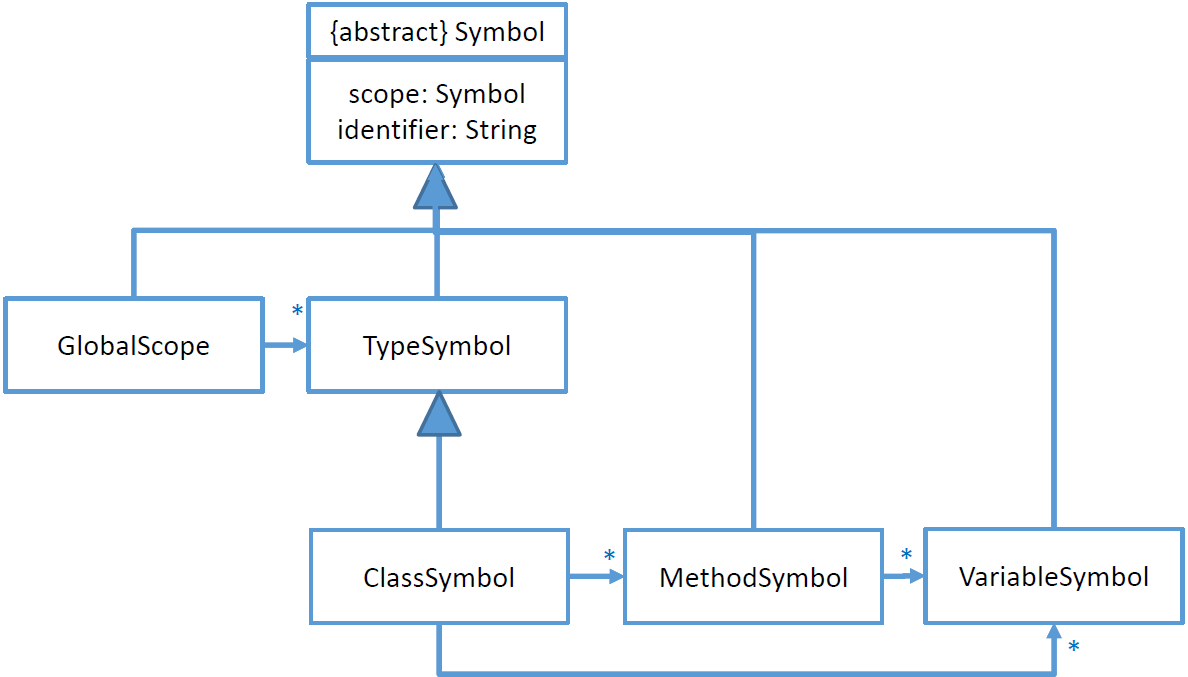
\includegraphics[width=0.7\linewidth]{symboltabelle_design.png}
\subsubsection{Detailiertere Beziehungen}
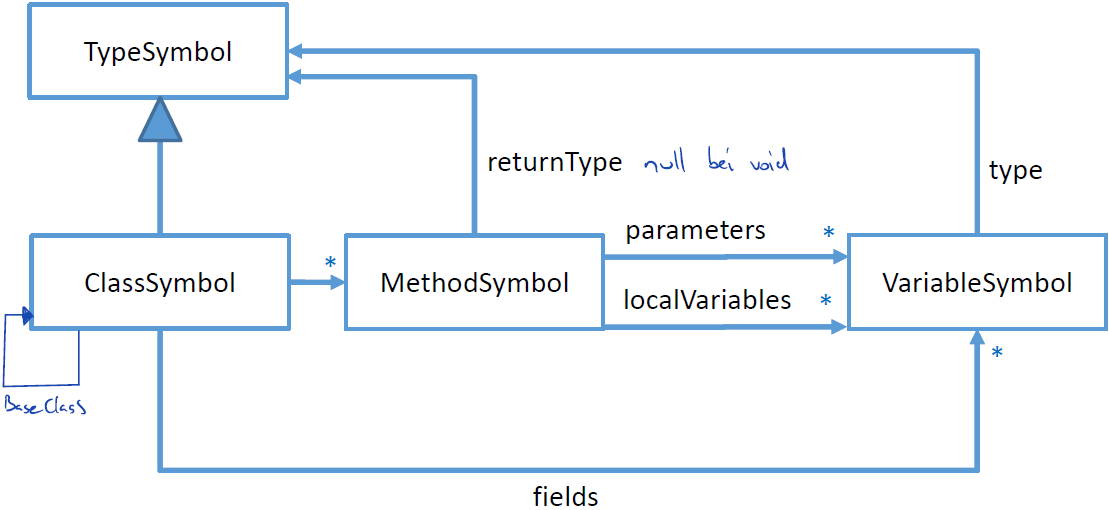
\includegraphics[width=0.7\linewidth]{symboltabelle_design_detailliert.png}
\subsubsection{Design Aspekte}
\textbf{Typinfo für Variable-Symbol}
\begin{itemize}
    \item Zuerst unaufgelöst (Identifier)
\end{itemize}
\textbf{Weitere Infos}
\begin{itemize}
    \item Klassen: Basisklasse
\end{itemize}
\textbf{Lokale Variablen}
\begin{itemize}
    \item Deklarationsbereich merken (Statements)
\end{itemize}
\textbf{Erweitertes Typ-Design}
\begin{itemize}
    \item Klassen
    \item Basistypen (int, boolean, string)
    \item Arrays
\end{itemize}
\textbf{Erweitertes Variablen-Design:}\\ 
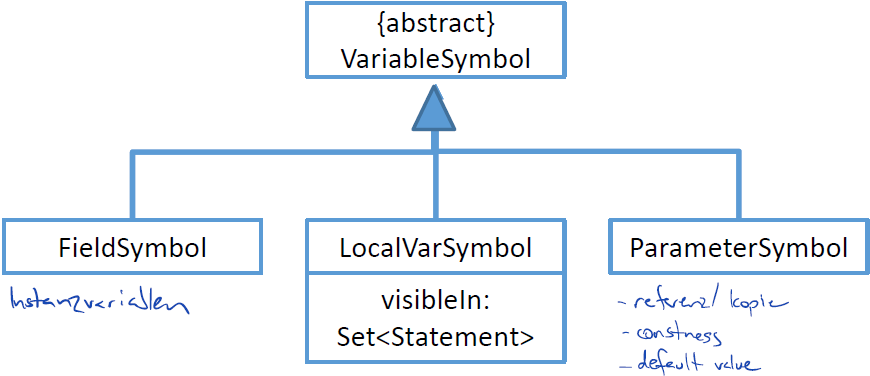
\includegraphics[width=0.5\linewidth]{var_design.png}
\subsubsection{AST Verknüpfung}
\begin{itemize}
    \item Symboltabelle enthält Mapping Symbol $\rightarrow$ AST
    \item Für alle Deklarationen
\end{itemize}
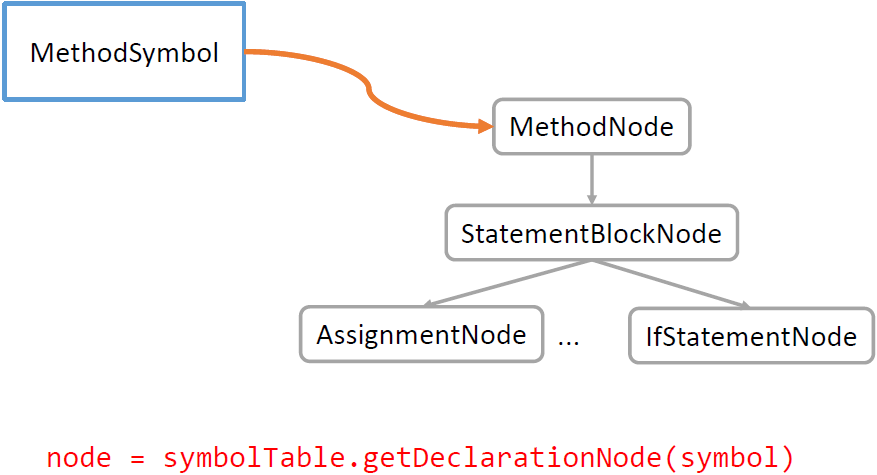
\includegraphics[width=0.6\linewidth]{ast_symboltabelle.png}

\subsection{Global Scope}
\begin{itemize}
    \item Mehrere Klassen im Programm
\end{itemize}

\subsection{Shadowing}
\begin{itemize}
    \item Deklarationen in inneren Bereichen verdecken gleichnamige von äusseren Bereichen
    \item Hiding: Bei gleicher Member-Name bei Vererbung
\end{itemize}

\subsection{Vorgehen}
\begin{enumerate}
    \item Konstruktion der Symboltabelle
    \item Typen in Tabelle auflösen 
    \item Deklaration in AST auflösen 
    \item Typen in AST auflösen
\end{enumerate}

\subsubsection{1. Konstruktion der Symboltabelle}
\textbf{AST traversieren}
\begin{itemize}
    \item Beginne mit Global Scope
    \item Pro Klasse, Methode, Parameter, Variable: Symbol in übergeordnetem Scope einfügen
    \item Explizit und/oder mit Visitor
\end{itemize}
\textbf{Forward-Referenzen $\rightarrow$ Typ-Namen und Designatoren noch nicht auflösen!}
\begin{itemize}
    \item Da vlt noch nicht alle Klassen in der Symboltabelle sind
\end{itemize}

\subsubsection{2. Typen in Tabelle auflösen}
\begin{itemize}
    \item Für Variablentype, Parametertyp, Rückgabetyp etc.
    \item Brauche Suche für Identifier auf Symboltabelle
    \begin{itemize}
        \item Starte mit innerstem Scope
        \item Suche stetig nach aussen ausbreiten
        \item Zuletzt in Global Scope suchen, ansonsten nicht vorhanden
    \end{itemize}
\end{itemize}
\begin{lstlisting}
Symbol find(Symbol scope, String identifier) {
    if(scope == null) {
        return null; // nicht im global scope
    }
    for (Symbol declaration : scope.allDeclarations()) {
        if(declaration.getIdentifier().equals(identifier)) {
            return declaration;
        }
    }
    return find(scope.getScope(), identifier); // rekursiv in nächst höheren Bereich
}
\end{lstlisting}

\subsubsection{3. Deklaration in AST auflösen}
\begin{itemize}
    \item Traversiere Ausführungscode in AST
    \item Jeden Designator auflösen, Deklaration zuordnen
\end{itemize}
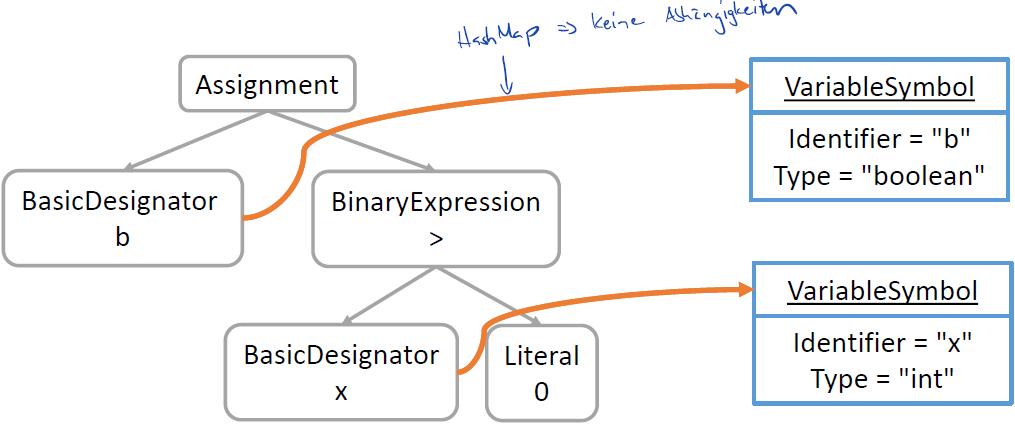
\includegraphics[width=0.7\linewidth]{dekl_in_ast.png}

\subsubsection{4. Typen in AST bestimmen}
\textbf{Typ zu jeder Expression zuordnen}
\begin{itemize}
    \item Literal: definierter Typ
    \item Designator: Typ der Deklaration
    \item Unary/BinaryExpression: Resultat des Operators
\end{itemize}
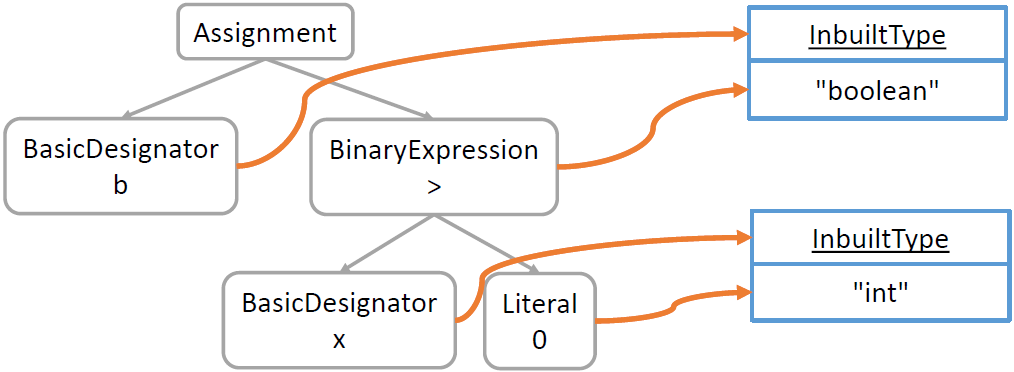
\includegraphics[width=0.7\linewidth]{typen_in_ast.png}\\
\textbf{Ablauf der Typenbestimmung:}
\begin{itemize}
    \item Post-Order-Traversierung
    \item AST am besten nicht erweitern sondern Maps in Symboltabelle verwenden
\end{itemize}
\subsubsection{Typauflösung per Visitor}
\begin{lstlisting}
@Override
public void visit(BinaryExpressionNode node) {
    Visitor.super.visit(node); // post-order travers
    var leftType = symboltable.findType(node.getLeft());
    var rightType = symboltable.findType(node.getRight());
    // ... 
    switch(node.getOperator()) {
        case PLUS -> {
            checkType(leftType, globalScope.getIntType());
            checkType(rightType, globalScope.getIntType());
            symboltable.fixType(node, globalScope.getIntType());
        }
        // ...
    }
}
\end{lstlisting}

\subsection{Semantic Checks}
\begin{itemize}
    \item Alle Designatoren beziehen sich auf Variablen/Methoden
    \item Typen stimmen bei Operatoren
    \item Kompatible Typen bei Zuweisungen
    \item Argumentliste passt auf Parameterliste
    \item Bedingungen in if, while sind boolean
    \item Return Ausdruck passt
    \item Keine Mehrfachdeklaration
    \item Kein Identifier ist reservierts Keyword
    \item Exakt eine main() Methode
    \item Array length  is read-only
    \item Kein Exit ohne Return (ausser void)
    \item Lesen von unitialisierten Variablen
    \item Null-Dereferenzierung
    \item Ungültiger Array-Index
    \item Division by Zero
    \item Out of Memory bei new()
\end{itemize}